\section{Performance}\label{sec:perf}

All micro-benchmarks were produced by \texttt{make bench} and \texttt{make
sizes} on the machine recorded in \texttt{results/bench\_env.json}: an
\texttt{arm64} macOS host, Python~3.15.2, \texttt{cryptography}~50.0.2 over
OpenSSL~4.0.3.

\subsection{P1: operation latency on the host}
\Cref{tab:bench} gives the median and 95th-percentile time of each operation over
10{,}000 runs (\texttt{results/bench.csv}). Every operation is cheap. ECDSA~P-256
signing is about $19\,\mu s$ and verification about $49\,\mu s$; the HMAC code is
about $5\,\mu s$. Ed25519 is shown for comparison only (it is not used by any
mode): it signs more slowly but with similarly small cost.

\begin{table}[htbp]
\centering
\caption{Operation latency on the host (P1, T7). Source:
\texttt{results/bench.csv}.}
\label{tab:bench}
\small
\begin{tabular}{@{}lrr@{}}
\toprule
Operation & Median ($\mu s$) & p95 ($\mu s$) \\
\midrule
\texttt{canonical\_encode}   & 3.50  & 3.71 \\
\texttt{totp}                & 1.62  & 1.75 \\
\texttt{hmac\_otp}           & 5.25  & 5.42 \\
\texttt{hmac\_otp\_verify}   & 5.42  & 5.58 \\
\texttt{ecdsa\_p256\_sign}   & 19.17 & 19.96 \\
\texttt{ecdsa\_p256\_verify} & 48.50 & 51.04 \\
\texttt{ed25519\_sign}       & 26.67 & 27.79 \\
\texttt{ed25519\_verify}     & 67.96 & 76.29 \\
\bottomrule
\end{tabular}
\end{table}

\begin{figure}[htbp]
\centering
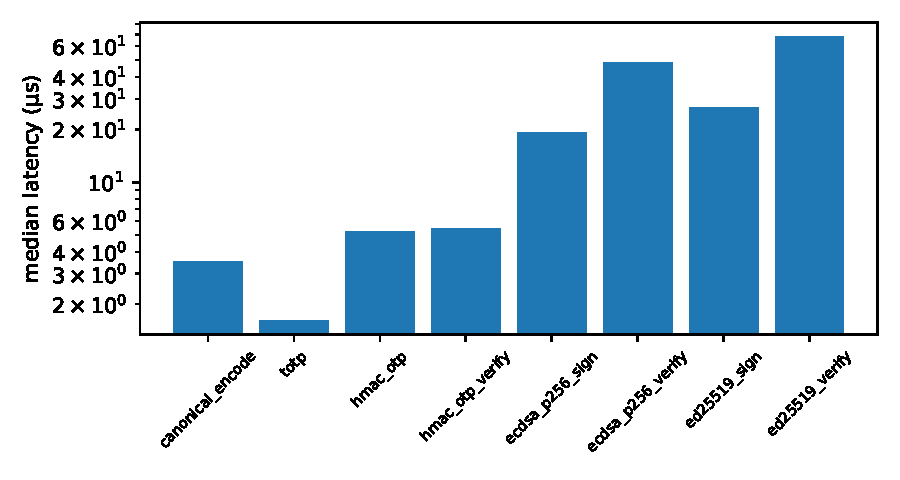
\includegraphics[width=0.75\linewidth]{figures/bench.pdf}
\caption{Operation latency on the host (F6).}
\label{fig:bench}
\end{figure}

\subsection{P2: signing on a real phone}
\Cref{tab:phone} reports the signing time measured in the authenticator itself on
two phones (200 signatures each, \texttt{results/phone\_bench.csv}). Safari on
iOS coarsens \texttt{performance.now()} to 1\,ms, so the per-sample median and
p95 read as 0 and 1\,ms and are not meaningful; the reliable figure is the mean
over the whole run, which is well under a millisecond on both devices. Signing
cost is therefore negligible next to the time the user spends scanning the QR and
reading the screen.

\begin{table}[htbp]
\centering
\caption{ECDSA P-256 signing on real phones (P2, T8). Source:
\texttt{results/phone\_bench.csv}. Median/p95 are limited by Safari's 1\,ms clock.}
\label{tab:phone}
\small
\begin{tabular}{@{}llrrrr@{}}
\toprule
Device & Browser & $n$ & Mean (ms) & Median (ms) & p95 (ms) \\
\midrule
iPhone Air & Safari 26.5 & 200 & 0.290 & 0.00 & 1.00 \\
iPhone 13  & Safari 26.4 & 200 & 0.415 & 0.00 & 1.00 \\
\bottomrule
\end{tabular}
\end{table}

\subsection{P3: data sizes}
\Cref{tab:sizes} lists the sizes that matter for the QR channel
(\texttt{results/sizes.csv}). A raw ECDSA~P-256 signature is 64~bytes (the same as
Ed25519), smaller than DER's 69--72~bytes, which is why the wire format is raw
$r\|s$. The canonical transaction is 199~bytes, giving a 271-character QR payload
at a version-12 symbol (error level~M) --- well within what a phone camera reads.

\begin{table}[htbp]
\centering
\caption{Data sizes (P3). Source: \texttt{results/sizes.csv}.}
\label{tab:sizes}
\small
\begin{tabular}{@{}lr@{}}
\toprule
Item & Value \\
\midrule
TOTP code (digits)                       & 6 \\
Transaction OTP (digits)                 & 8 \\
ECDSA P-256 signature, raw (bytes)       & 64 \\
ECDSA P-256 signature, DER min/max (bytes)& 69 / 72 \\
Ed25519 signature (bytes)                & 64 \\
Canonical transaction (bytes)            & 199 \\
QR payload (characters)                  & 271 \\
QR version (error level M)               & 12 \\
\bottomrule
\end{tabular}
\end{table}

\paragraph{On usability.}
A planned timing study (P4: completion time over seven participants) was dropped
from scope. The report therefore makes no usability-timing claim; the usability
discussion is confined to the qualitative cost of scanning and reading, and to
the attentive-user limitation already stated.
